\documentclass[crop,tikz]{standalone}
\usepackage{tikz}

\usetikzlibrary{positioning}

\definecolor{olivegreen}{rgb}{0,0.6,0}
\definecolor{mymauve}{rgb}{0.58,0,0.82}
\definecolor{camdrk}{RGB}{0,62,114}

\begin{document}
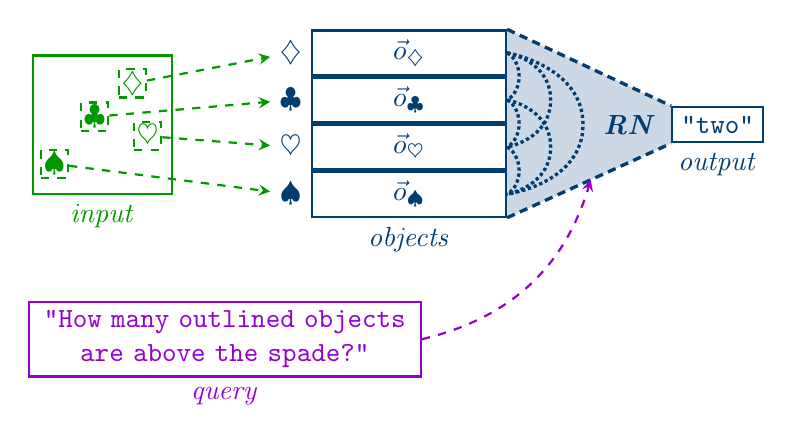
\begin{tikzpicture}
	\node[rectangle, draw, thick, olivegreen, minimum width=5em, minimum height=5em] (R) at (0, 0) {};
	\node[rectangle, inner sep=0.1em, olivegreen,dashed, draw, thick] (C) at (-0.1, 0.1) {$\clubsuit$};
	\node[rectangle, thick, inner sep=0.1em, olivegreen,dashed, draw, above right=0.1em and 0.3em of C] (D) {$\diamondsuit$};
	\node[rectangle, thick, inner sep=0.1em, olivegreen,dashed, draw, below right=0.8em and -0.5em of D] (H) {$\heartsuit$};
	\node[rectangle, thick, inner sep=0.1em, olivegreen,dashed, draw, below left=0.6em and 0.4em of C] (S) {$\spadesuit$};
	\node[olivegreen,below=0em of R] (l1) {\emph{input}};
		
	\node[camdrk, rectangle, draw, above right=-2.5em and 5em of R, minimum width=7em, thick]  (Oc) {$\vec{o}_\clubsuit$};
	\node[camdrk, rectangle, draw, above=0em of Oc, minimum width=7em, thick]  (Od) {$\vec{o}_\diamondsuit$};
	\node[camdrk, rectangle, draw, below=0em of Oc, minimum width=7em, thick]  (Oh) {$\vec{o}_\heartsuit$};
	\node[camdrk, rectangle, draw, below=0em of Oh, minimum width=7em, thick]  (Os) {$\vec{o}_\spadesuit$};
		
	\node[camdrk, left=0em of Oc] (lc) {$\clubsuit$};
	\node[camdrk, left=0em of Od] (ld) {$\diamondsuit$};
	\node[camdrk, left=0em of Oh] (lh) {$\heartsuit$};
	\node[camdrk, left=0em of Os] (ls) {$\spadesuit$};
		
	\node[camdrk, below=0em of Os] (lr) {\emph{objects}};
		
	\draw[olivegreen,-stealth, thick, dashed] (C) -- (lc);
	\draw[olivegreen,-stealth, thick, dashed] (D) -- (ld);
	\draw[olivegreen,-stealth, thick, dashed] (H) -- (lh);
	\draw[olivegreen,-stealth, thick, dashed] (S) -- (ls);
		
	\node[draw, camdrk, thick, right=18em of R] (A) {\texttt{"two"}};
	\node[camdrk, below=0em of A] {\emph{output}};
		
	\draw[camdrk, densely dashed, very thick] (Od.north east) -- (A.north west);
	\draw[camdrk, densely dashed, very thick] (Os.south east) -- (A.south west);
		
	\fill [opacity=0.2, camdrk] (Od.north east) -- (A.north west) -- (A.south west) -- (Os.south east) -- cycle;
		
	% let's get funky
	\node[right=14.75em of R, inner sep=0em] (dum1) {};
	\node[right=1.5em of Oc, inner sep=0em] (dum2) {};
	\node[right=1.5em of Oh, inner sep=0em] (dum3) {};
		
	\draw[camdrk, densely dotted, very thick] (Od.east) edge[bend left=60] (Oc.east);
	\draw[camdrk, densely dotted, very thick] plot [smooth, tension=1.5] coordinates { (Od.east) (dum2) (Oh.east)};
	\draw[camdrk, densely dotted, very thick] plot [smooth, tension=1.5] coordinates { (Od.east) (dum1) (Os.east)};
	\draw[camdrk, densely dotted, very thick] (Oc.east) edge[bend left=60] (Oh.east);
	\draw[camdrk, densely dotted, very thick] plot [smooth, tension=1.5] coordinates { (Oc.east) (dum3) (Os.east)};
	\draw[camdrk, densely dotted, very thick] (Oh.east) edge[bend left=60] (Os.east);
		
	\node[mymauve,rectangle, thick, align=center, draw, below left=3em and -4em of Os, text width=13.5em] (Q) {\texttt{"How many outlined objects are above the spade?"}};
	\node[mymauve,below=0em of Q] (ql) {\emph{query}};
		
	\path[mymauve,-stealth, dashed, thick] (Q.east) edge[bend right] (6.2, -0.7);
		
	\node[camdrk] at (6.7, 0) (RN){\textbf{\emph{RN}}};
		
\end{tikzpicture}
\end{document}